% !TeX program = xelatex
% 编译方式：XeLaTeX（建议连续编译两次以更新交叉引用）
\documentclass[UTF8,12pt,a4paper]{ctexart}

% ==================== 基础宏包 ====================
\usepackage[left=2.4cm,right=2.4cm,top=2.5cm,bottom=2.5cm]{geometry}
\usepackage{amsmath,amssymb,amsthm,mathtools,bm}
\usepackage{booktabs,array,multirow}
\usepackage{enumitem}
\usepackage{algorithm}
\usepackage{algpseudocode}
\usepackage{graphicx}
\usepackage{subcaption}
\usepackage{xcolor}
\usepackage{tikz}
\usetikzlibrary{arrows.meta,calc,positioning,angles,quotes,patterns,decorations.pathreplacing}
\usepackage{hyperref}
\usepackage[nameinlink,noabbrev]{cleveref}

% ==================== 颜色与版式 ====================
\definecolor{mainblue}{RGB}{42,92,145}
\definecolor{maingreen}{RGB}{55,125,92}
\definecolor{mainred}{RGB}{180,65,60}
\definecolor{mainorange}{RGB}{210,130,45}
\definecolor{lightblue}{RGB}{225,237,248}
\definecolor{lightgreen}{RGB}{227,242,232}
\definecolor{lightred}{RGB}{250,230,228}
\hypersetup{
  colorlinks=true,
  linkcolor=mainblue,
  citecolor=maingreen,
  urlcolor=mainblue
}
\setlength{\parindent}{2em}
\setlength{\parskip}{0.25em}
\setlist[itemize]{leftmargin=2em}
\setlist[enumerate]{leftmargin=2.2em}

% ==================== 定理环境 ====================
\newtheorem{theorem}{定理}[section]
\newtheorem{lemma}[theorem]{引理}
\newtheorem{proposition}[theorem]{命题}
\newtheorem{corollary}[theorem]{推论}
\theoremstyle{definition}
\newtheorem{definition}[theorem]{定义}
\newtheorem{remark}[theorem]{说明}
\renewcommand{\proofname}{证明}

% cleveref 中文名称
\crefname{figure}{图}{图}
\crefname{table}{表}{表}
\crefname{equation}{式}{式}
\crefname{algorithm}{算法}{算法}
\crefname{theorem}{定理}{定理}
\crefname{lemma}{引理}{引理}
\crefname{proposition}{命题}{命题}
\crefname{corollary}{推论}{推论}
\crefname{definition}{定义}{定义}
\crefname{remark}{说明}{说明}

% ==================== 常用数学符号 ====================
\newcommand{\R}{\mathbb{R}}
\newcommand{\eps}{\varepsilon}
\newcommand{\norm}[1]{\left\lVert #1\right\rVert}
\newcommand{\abs}[1]{\left\lvert #1\right\rvert}
\newcommand{\cross}{\mathbin{\times}}
\DeclareMathOperator{\conv}{conv}
\DeclareMathOperator{\MEC}{MEC}
\DeclareMathOperator*{\argmax}{arg\,max}
\DeclareMathOperator*{\argmin}{arg\,min}

% algorithmic 中文化
\algrenewcommand\algorithmicrequire{\textbf{输入：}}
\algrenewcommand\algorithmicensure{\textbf{输出：}}
\algrenewcommand\algorithmiccomment[1]{\hfill$\triangleright$~#1}

\title{问题一：基于半平面交、旋转卡壳与 Welzl 算法的\\定位区域直径计算与覆盖性判定}
\author{}
\date{}

\begin{document}
\maketitle
\tableofcontents
\newpage

% ============================================================
\section{问题描述与总体建模思路}
% ============================================================

设第 $i$ 个检测点的位置为
\[
S_i=(x_i,y_i),\qquad i=1,2,\ldots,N,
\]
其测得的干扰源示向角为 $\theta_i$，测角误差上限为 $\eps$（题设中可取 $\eps=1^\circ$）。由于测角误差的存在，单个检测点给出的并非一条精确射线，而是一个方向区间
\begin{equation}
\theta_i-\eps\leq \arg(P-S_i)\leq \theta_i+\eps,
\label{eq:angle-interval}
\end{equation}
其中 $P=(x,y)$ 表示干扰源可能位置。

当 $2\eps<180^\circ$ 时，\cref{eq:angle-interval} 对应一个凸角域，而一个凸角域可以表示为两个半平面的交。因此，多个检测点共同产生的定位区域可以写成有限个半平面的公共部分
\begin{equation}
\Omega=\bigcap_{j=1}^{n}H_j,
\label{eq:omega-hpi}
\end{equation}
其中 $n=2N$（若还存在其他线性先验约束，则相应增加半平面个数）。

本问进一步需要求定位区域的直径
\begin{equation}
D=\max_{P,Q\in\Omega}\norm{P-Q},
\label{eq:diameter-def}
\end{equation}
以及判断是否存在一个\emph{直径恰为 $D$} 的圆能够完整覆盖 $\Omega$。

综合考虑几何结构与计算复杂度，采用如下算法链：
\begin{equation}
\boxed{
\text{示向角约束}
\longrightarrow
\text{半平面交 HPI}
\longrightarrow
\text{凸多边形}
\longrightarrow
\begin{cases}
\text{旋转卡壳求 }D,\\
\text{Welzl 求 }R^*,
\end{cases}
\longrightarrow
\rho=\dfrac{2R^*}{D}
}
\label{eq:overall-pipeline}
\end{equation}
其中 $R^*$ 为定位区域的最小覆盖圆半径。

\begin{figure}[htbp]
\centering
\begin{tikzpicture}[
  node distance=8mm and 7mm,
  box/.style={draw=mainblue,rounded corners=2mm,fill=lightblue,minimum height=10mm,minimum width=28mm,align=center,font=\small},
  box2/.style={draw=maingreen,rounded corners=2mm,fill=lightgreen,minimum height=10mm,minimum width=30mm,align=center,font=\small},
  arr/.style={-{Latex[length=2.4mm]},thick,draw=gray!75}
]
\node[box] (a) {示向角\\$\theta_i\pm\eps$};
\node[box,right=of a] (b) {角域转化为\\两个半平面};
\node[box,right=of b] (c) {半平面交\\HPI};
\node[box,right=of c] (d) {凸多边形\\$V_1,\ldots,V_m$};
\node[box2,above right=5mm and 12mm of d] (e) {旋转卡壳\\直径 $D$};
\node[box2,below right=5mm and 12mm of d] (f) {Welzl\\最小半径 $R^*$};
\node[box,right=24mm of d] (g) {计算\\$\rho=2R^*/D$};
\draw[arr] (a)--(b);
\draw[arr] (b)--(c);
\draw[arr] (c)--(d);
\draw[arr] (d.east) -- ++(7mm,0) |- (e.west);
\draw[arr] (d.east) -- ++(7mm,0) |- (f.west);
\draw[arr] (e.east) -- ++(6mm,0) |- (g.north west);
\draw[arr] (f.east) -- ++(6mm,0) |- (g.south west);
\end{tikzpicture}
\caption{问题一的总体求解流程。半平面交负责恢复定位区域，旋转卡壳与 Welzl 算法分别计算区域直径和最小覆盖圆。}
\label{fig:pipeline}
\end{figure}

% ============================================================
\section{示向角约束的半平面化}
% ============================================================

\subsection{有向直线与半平面判定}

设一条有向直线经过点 $S=(x_s,y_s)$，方向角为 $\alpha$，对应方向向量
\begin{equation}
\bm d=(\cos\alpha,\sin\alpha).
\end{equation}
统一规定有向直线的\textbf{左侧为可行半平面}。对于任意点 $P=(x,y)$，有
\begin{equation}
P\in H
\quad\Longleftrightarrow\quad
\bm d\cross(P-S)\geq 0,
\label{eq:left-halfplane-cross}
\end{equation}
其中二维叉积定义为
\begin{equation}
(a_x,a_y)\cross(b_x,b_y)=a_xb_y-a_yb_x.
\end{equation}
展开\cref{eq:left-halfplane-cross} 可得
\begin{align}
&\cos\alpha(y-y_s)-\sin\alpha(x-x_s)\geq0,\\
\Longleftrightarrow\quad
&\sin\alpha\,x-\cos\alpha\,y
\leq
\sin\alpha\,x_s-\cos\alpha\,y_s.
\label{eq:halfplane-linear}
\end{align}
因此每一条有向边界均可化为标准线性半平面 $Ax+By\leq C$。

\subsection{一个示向角对应两个半平面}

对检测点 $S_i$，定义上下边界方向向量
\begin{equation}
\bm d_i^-=
\bigl(\cos(\theta_i-\eps),\sin(\theta_i-\eps)\bigr),
\end{equation}
\begin{equation}
\bm d_i^+=
\bigl(\cos(\theta_i+\eps),\sin(\theta_i+\eps)\bigr).
\end{equation}
若允许角域由 $\bm d_i^-$ 逆时针旋转至 $\bm d_i^+$，则
\begin{equation}
W_i=
\left\{P:\bm d_i^-\cross(P-S_i)\geq0\right\}
\cap
\left\{P:\bm d_i^+\cross(P-S_i)\leq0\right\}.
\label{eq:wedge-two-hp}
\end{equation}
将第二条边界方向反转，即可继续统一使用“左侧为可行域”的表示。

\begin{figure}[htbp]
\centering
\begin{tikzpicture}[scale=1.05,>=Latex]
  \coordinate (S) at (0,0);
  \fill[mainblue!13] (S) -- (18:4.5) arc[start angle=18,end angle=52,radius=4.5] -- cycle;
  \draw[-{Latex[length=3mm]},very thick,mainblue] (S)--(18:5.0) node[right] {$\bm d_i^-$};
  \draw[-{Latex[length=3mm]},very thick,maingreen] (S)--(52:5.0) node[above right] {$\bm d_i^+$};
  \draw[dashed,gray] (S)--(35:5.1);
  \node[below left] at (S) {$S_i$};
  \fill (S) circle (1.6pt);
  \draw[->,mainorange,thick] (1.15,0.15) arc[start angle=8,end angle=34,radius=1.15];
  \node[mainorange] at (1.55,0.63) {$2\eps$};
  \node[mainblue!80!black,align=center] at (3.0,2.0) {允许角域 $W_i$\\$=H_i^-\cap H_i^+$};
  \node[gray!80] at (3.9,0.65) {$\theta_i-\eps$};
  \node[gray!80] at (3.35,3.1) {$\theta_i+\eps$};
\end{tikzpicture}
\caption{示向角误差区间的几何表示。一个小于 $180^\circ$ 的角域可严格表示为两个半平面的交。}
\label{fig:wedge-halfplanes}
\end{figure}

\subsection{定位区域的凸性}

\begin{lemma}[定位区域凸性]
由有限个半平面定义的定位区域 $\Omega=\bigcap_{j=1}^nH_j$ 为凸集；若其非空且有界，则 $\Omega$ 为凸多边形。
\end{lemma}
\begin{proof}
任取 $X,Y\in H_j$ 以及 $\lambda\in[0,1]$，由叉积对向量的线性性，
\begin{align}
\bm d_j\cross\bigl(\lambda X+(1-\lambda)Y-S_j\bigr)
&=\lambda\bm d_j\cross(X-S_j)\\
&\quad +(1-\lambda)\bm d_j\cross(Y-S_j)\geq0.
\end{align}
故每个 $H_j$ 均为凸集。凸集的任意交仍为凸集，因此 $\Omega$ 为凸集。若 $\Omega$ 非空、有界且由有限条直线约束，则其边界由有限条线段组成，故为凸多边形。
\end{proof}

% ============================================================
\section{双端队列半平面交算法}
% ============================================================

\subsection{直线交点公式}

设两条有向直线为
\begin{equation}
L_1:P_1+t\bm d_1,
\qquad
L_2:P_2+s\bm d_2.
\end{equation}
若 $\bm d_1\cross\bm d_2\neq0$，由
\[
P_1+t\bm d_1=P_2+s\bm d_2
\]
两侧与 $\bm d_2$ 做叉积，可得
\begin{equation}
t=
\frac{(P_2-P_1)\cross\bm d_2}
{\bm d_1\cross\bm d_2},
\end{equation}
故交点为
\begin{equation}
\boxed{
I(L_1,L_2)
=P_1+
\frac{(P_2-P_1)\cross\bm d_2}
{\bm d_1\cross\bm d_2}\bm d_1.
}
\label{eq:line-intersection}
\end{equation}
若 $\abs{\bm d_1\cross\bm d_2}<\eps_{\rm num}$，则两直线视为平行并进行特殊处理。

\subsection{方向角排序与同向去重}

令
\begin{equation}
\alpha_j=\operatorname{atan2}(d_{jy},d_{jx})\in[0,2\pi).
\end{equation}
将所有半平面按 $\alpha_j$ 递增排序。若若干半平面方向相同，设其共同左法向量为 $\bm n=(-d_y,d_x)$，则可统一写成
\begin{equation}
\bm n\cdot P\geq c_k.
\end{equation}
显然只有最大的 $c_k$ 有效，因此同方向约束只保留最严格者
\begin{equation}
c=\max_k c_k.
\end{equation}

\subsection{双端队列维护}

\begin{algorithm}[htbp]
\caption{双端队列半平面交（HPI）}
\label{alg:hpi}
\begin{algorithmic}[1]
\Require 半平面集合 $\mathcal H=\{H_1,\ldots,H_n\}$，所有边界均统一为“左侧可行”
\Ensure 半平面交凸多边形顶点 $V_1,\ldots,V_m$
\State 按边界方向角对 $\mathcal H$ 排序，并删除同方向冗余约束
\State 初始化双端队列 $Q\gets\varnothing$
\For{每个半平面 $H$（按方向角顺序）}
    \While{$|Q|\ge2$ 且 $I(Q_{-2},Q_{-1})\notin H$}
        \State $Q.\mathrm{pop\_back}()$
    \EndWhile
    \While{$|Q|\ge2$ 且 $I(Q_0,Q_1)\notin H$}
        \State $Q.\mathrm{pop\_front}()$
    \EndWhile
    \State $Q.\mathrm{push\_back}(H)$
\EndFor
\While{$|Q|\ge3$ 且 $I(Q_{-2},Q_{-1})\notin Q_0$}
    \State $Q.\mathrm{pop\_back}()$
\EndWhile
\While{$|Q|\ge3$ 且 $I(Q_0,Q_1)\notin Q_{-1}$}
    \State $Q.\mathrm{pop\_front}()$
\EndWhile
\For{$i=1,\ldots,m-1$}
    \State $V_i\gets I(Q_i,Q_{i+1})$
\EndFor
\State $V_m\gets I(Q_m,Q_1)$
\State \Return $V_1,\ldots,V_m$
\end{algorithmic}
\end{algorithm}

\subsection{为什么新半平面只会删除连续的一段边界}

\begin{lemma}[连续切割性]
设当前可行域 $\Omega_k$ 为凸多边形，加入新半平面 $H$ 后，$\Omega_{k+1}=\Omega_k\cap H$。则被 $H$ 删除的 $\partial\Omega_k$ 部分必为一段连续边界链（允许为空）。
\label{lem:continuous-cut}
\end{lemma}
\begin{proof}
新半平面边界 $L=\partial H$ 与凸集 $\Omega_k$ 的交仍为凸集，因此 $L\cap\Omega_k$ 只能是空集、单点或线段。也就是说，沿 $L$ 观察时，它至多穿入、穿出凸区域各一次。若被删除的边界包含两段互不相连的链，则 $L$ 必须在凸区域内外之间至少交替两次以上，与 $L\cap\Omega_k$ 为凸集矛盾。因此被删除部分必连续。
\end{proof}

\subsection{队尾弹出的几何证明}

设当前 deque 尾部为 $\cdots,A,B$，新加入半平面为 $H_C$。旧尾部候选顶点为
\begin{equation}
X=A\cap B.
\end{equation}
若
\begin{equation}
X\notin H_C,
\label{eq:tail-outside}
\end{equation}
则旧顶点 $X$ 被新半平面切掉。

\begin{lemma}[队尾弹出正确性]
在半平面边界按方向角递增处理、deque 已正确表示当前凸边界链的前提下，若\cref{eq:tail-outside} 成立，则队尾边界 $B$ 不可能继续成为新区域 $\Omega_k\cap H_C$ 的有效边界，故可执行 $\mathrm{pop\_back}(B)$。
\label{lem:pop-back}
\end{lemma}
\begin{proof}
由\cref{lem:continuous-cut}，$H_C$ 对旧凸边界的删除只能形成一段连续链。又由于 $C$ 是当前扫描中方向角最大的边界之一，它首先接触的是方向角序列的尾端。既然尾部顶点 $A\cap B$ 已落在 $H_C$ 外，则与该顶点相连且位于扫描尾端的旧边界 $B$ 已进入被删除的连续边界链；它不再可能在新的凸区域边界上保留正长度线段。因此 $B$ 不再是有效支撑边，可以安全删除。删除后若新的尾部交点仍在 $H_C$ 外，则同理继续删除，直至边界链重新进入 $H_C$。
\end{proof}

\begin{figure}[htbp]
\centering
\begin{tikzpicture}[scale=0.95,>=Latex]
% ---------- 左侧几何图 ----------
\begin{scope}[xshift=-4.3cm]
  \node[font=\bfseries] at (0,3.25) {(a) 几何含义};
  % 新半平面填充（示意）
  \fill[maingreen!10] (-3.2,2.7) -- (2.8,2.7) -- (2.8,0.15) -- (-3.2,-1.55) -- cycle;
  % 三条线
  \draw[very thick,mainblue,-{Latex[length=2.4mm]}] (-2.8,2.4)--(1.1,-1.1) node[pos=0.15,left] {$A$};
  \draw[very thick,mainorange,-{Latex[length=2.4mm]}] (-2.7,-0.15)--(2.4,-0.15) node[pos=0.86,below] {$B$};
  \draw[very thick,maingreen,-{Latex[length=2.4mm]}] (-2.9,-1.45)--(2.55,0.3) node[pos=0.88,above] {$C$};
  % X intersection approx A with B at (0.1,-0.15)
  \fill[mainred] (0.02,-0.15) circle (2.3pt);
  \node[mainred,above right] at (0.02,-0.15) {$X=A\cap B$};
  \draw[mainred,thick,-{Latex[length=2mm]}] (0.55,1.25)--(0.12,0.05);
  \node[mainred,align=center] at (1.15,1.65) {$X\notin H_C$\\旧顶点被切掉};
  \node[maingreen!70!black] at (-1.6,2.15) {$H_C$ 可行侧};
  \draw[decorate,decoration={brace,amplitude=5pt},mainred] (-0.2,-0.43)--(1.75,-0.43)
     node[midway,below=6pt,align=center] {$B$ 的尾部边界\\不再有效};
\end{scope}
% ---------- 右侧 deque 图 ----------
\begin{scope}[xshift=4.1cm]
  \node[font=\bfseries] at (0,3.25) {(b) deque 的变化};
  \node at (-2.3,1.55) {加入 $C$ 前：};
  \foreach \x/\txt/\col in {-0.9/$\cdots$/gray!55,0.25/$A$/mainblue,1.4/$B$/mainorange}{
    \node[draw=\col,very thick,rounded corners=1.5mm,minimum width=10mm,minimum height=8mm] at (\x,1.55) {\txt};
  }
  \node[mainred] at (2.35,1.55) {$X\notin H_C$};
  \draw[mainred,very thick] (1.15,1.25)--(1.65,1.85);
  \draw[mainred,very thick] (1.15,1.85)--(1.65,1.25);
  \node at (-2.25,0.15) {弹出 $B$：};
  \foreach \x/\txt/\col in {-0.9/$\cdots$/gray!55,0.25/$A$/mainblue}{
    \node[draw=\col,very thick,rounded corners=1.5mm,minimum width=10mm,minimum height=8mm] at (\x,0.15) {\txt};
  }
  \node[draw=maingreen,very thick,rounded corners=1.5mm,minimum width=10mm,minimum height=8mm] at (1.4,0.15) {$C$};
  \draw[-{Latex[length=2.5mm]},thick,gray] (0.55,0.85)--(0.55,0.5);
  \node[align=center,text width=6.5cm] at (0,-1.25) {由于凸性，新半平面只能连续切掉旧边界的一段；\\方向角排序后，这段失效边界只能从 deque 两端连续出现。};
\end{scope}
\end{tikzpicture}
\caption{双端队列队尾弹出的证明示意。当新半平面 $H_C$ 排除旧尾部顶点 $X=A\cap B$ 时，$B$ 已进入被连续切掉的边界链，因此可安全执行 $\mathrm{pop\_back}$。}
\label{fig:pop-back-proof}
\end{figure}

\subsection{为什么还需要 \texorpdfstring{$\mathrm{pop\_front}$}{pop-front}}

方向角本质上是模 $2\pi$ 的循环变量，即 $0\equiv2\pi$。因此例如 $350^\circ$ 与 $10^\circ$ 在数组中位于两端，但在几何方向上实际相邻。由\cref{lem:continuous-cut}，一段连续失效边界若跨越人为设置的 $0/2\pi$ 切口，在线性 deque 中就表现为“队尾一段 + 队首一段”。故还必须检查
\[
I(Q_0,Q_1)\in H_C?
\]
若不成立，则对循环方向重新编号后与\cref{lem:pop-back} 完全同构，应执行 $\mathrm{pop\_front}$。

\subsection{半平面交算法的全局正确性}

\begin{theorem}[HPI 正确性]
设所有半平面边界已统一为左侧可行，并按方向角排序、去除同向冗余约束。若最终半平面交非空且有界，则\cref{alg:hpi} 返回的相邻直线交点按循环顺序恰好构成 $\Omega$ 的全部顶点。
\label{thm:hpi-correct}
\end{theorem}
\begin{proof}
对已处理半平面的数量 $k$ 做归纳。假设处理前 $k$ 个半平面后，deque 按方向角保存当前凸区域 $\Omega_k$ 的有效边界链。加入 $H_{k+1}$ 后，由\cref{lem:continuous-cut}，旧边界中失效部分只能是一段连续链；在线性 deque 中只能从尾端或跨越角度切口后同时从首尾两端出现。\cref{lem:pop-back} 及其队首对称情形保证两个 while 循环恰好删除全部失效边界而不删除有效边界，再把新支撑边 $H_{k+1}$ 入队，即得到 $\Omega_{k+1}$ 的有效边界链。因此归纳成立。

全部半平面处理完毕后，最终首尾检查恢复 $0/2\pi$ 处的循环相邻关系。此时 deque 中每条直线均为最终凸区域的有效支撑边，相邻两条支撑边的交点必为一个顶点；反之，凸多边形每个顶点必由两条相邻有效支撑边相交得到。因此返回的顶点既不多也不少，恰为 $\Omega$ 的全部顶点。
\end{proof}

\subsection{HPI 时间复杂度}

方向角排序需要 $O(n\log n)$；同向去重只需一次线性扫描。队列维护中每条直线最多入队一次、出队一次，因此所有 $\mathrm{pop\_front}$ 与 $\mathrm{pop\_back}$ 的总次数为 $O(n)$。于是
\begin{equation}
\boxed{T_{\rm HPI}(n)=O(n\log n)},
\end{equation}
空间复杂度为 $O(n)$。

% ============================================================
\section{旋转卡壳求凸多边形直径}
% ============================================================

设 HPI 得到按逆时针排列的凸多边形顶点
\[
V_0,V_1,\ldots,V_{m-1}.
\]

\subsection{直径必可由顶点对取得}

\begin{proposition}
凸多边形 $\Omega$ 的直径可写成
\begin{equation}
D=\max_{0\le i,j<m}\norm{V_i-V_j}.
\label{eq:diameter-vertices}
\end{equation}
\end{proposition}
\begin{proof}
固定 $Q\in\Omega$，函数 $f(P)=\norm{P-Q}$ 为凸函数。凸函数在紧凸多边形上的最大值至少可在极点（顶点）处取得，故对该 $Q$ 存在顶点 $V_i$ 达到最远距离。再固定 $V_i$ 对 $Q$ 做同样论证，可将另一端也取为某个顶点 $V_j$。因此\cref{eq:diameter-vertices} 成立。
\end{proof}

\subsection{对踵点与旋转卡壳}

对固定边 $E_i=V_iV_{i+1}$，顶点 $V_j$ 到该边所在直线的距离为
\begin{equation}
h_i(j)=
\frac{
\abs{(V_{i+1}-V_i)\cross(V_j-V_i)}
}{\norm{V_{i+1}-V_i}}.
\label{eq:edge-point-distance}
\end{equation}
固定 $i$ 时分母不变，因此寻找最远支撑点等价于最大化叉积绝对值
\begin{equation}
A_i(j)=\abs{(V_{i+1}-V_i)\cross(V_j-V_i)},
\label{eq:area-objective}
\end{equation}
它等于三角形 $\triangle V_iV_{i+1}V_j$ 面积的两倍。

\begin{definition}[对踵对]
若存在两条互相平行的支撑线分别接触凸多边形的两个顶点或边，并将整个凸多边形夹在二者之间，则对应的接触对象称为一组对踵对（antipodal pair）。
\end{definition}

\begin{figure}[htbp]
\centering
\begin{tikzpicture}[scale=1.05,>=Latex]
  \coordinate (v0) at (-2.8,-1.25);
  \coordinate (v1) at (0.8,-1.25);
  \coordinate (v2) at (2.5,-0.2);
  \coordinate (v3) at (1.25,1.75);
  \coordinate (v4) at (-0.7,2.15);
  \coordinate (v5) at (-2.6,0.75);
  \fill[mainblue!7] (v0)--(v1)--(v2)--(v3)--(v4)--(v5)--cycle;
  \draw[thick] (v0)--(v1)--(v2)--(v3)--(v4)--(v5)--cycle;
  \draw[very thick,mainblue] (v0)--(v1);
  \draw[dashed,very thick,mainorange] (-3.3,-1.25)--(3.0,-1.25);
  \draw[dashed,very thick,mainorange] (-3.3,2.15)--(3.0,2.15);
  \fill[mainred] (v4) circle (2.5pt);
  \node[above] at (v4) {$V_j$};
  \fill[mainblue] (v0) circle (2pt) node[below left] {$V_i$};
  \fill[mainblue] (v1) circle (2pt) node[below] {$V_{i+1}$};
  \draw[<->,mainred,thick] (0.1,-1.14)--(0.1,2.04) node[midway,right] {$h_i(j)$};
  \draw[->,maingreen,thick] (3.15,-0.65) arc[start angle=-70,end angle=-15,radius=1.0];
  \draw[->,maingreen,thick] (3.15,1.55) arc[start angle=110,end angle=165,radius=1.0];
  \node[maingreen!70!black,align=center] at (4.0,0.45) {两条平行支撑线\\同步旋转};
  \node[mainorange!80!black] at (-4.1,2.15) {支撑线};
  \node[mainorange!80!black] at (-4.1,-1.25) {支撑线};
\end{tikzpicture}
\caption{旋转卡壳示意。固定一条多边形边 $V_iV_{i+1}$ 后，另一条平行支撑线接触最远点 $V_j$；随着边方向单调旋转，接触点也只沿凸边界单向前进。}
\label{fig:rotating-calipers}
\end{figure}

\subsection{为什么直径点对一定是对踵点}

\begin{lemma}[直径点对的支撑性]
若 $P,Q\in\Omega$ 满足 $\norm{P-Q}=D$，则存在两条互相平行、分别经过 $P,Q$ 的支撑线；故 $(P,Q)$ 必属于某组对踵关系。
\label{lem:diameter-antipodal}
\end{lemma}
\begin{proof}
令
\[
\bm u=\frac{P-Q}{D}.
\]
若存在 $X\in\Omega$ 满足 $(X-P)\cdot\bm u>0$，则
\begin{align}
\norm{X-Q}^2
&=\norm{(P-Q)+(X-P)}^2\\
&=D^2+2D\,\bm u\cdot(X-P)+\norm{X-P}^2\\
&>D^2,
\end{align}
即 $\norm{X-Q}>D$，与 $D$ 为直径矛盾。因此所有 $X\in\Omega$ 均满足 $(X-P)\cdot\bm u\le0$，说明经过 $P$ 且法向量为 $\bm u$ 的直线为支撑线。同理经过 $Q$ 的平行直线也是支撑线，故 $(P,Q)$ 为对踵对。
\end{proof}

\subsection{旋转卡壳算法}

\begin{algorithm}[htbp]
\caption{旋转卡壳求凸多边形直径}
\label{alg:calipers}
\begin{algorithmic}[1]
\Require 逆时针凸多边形顶点 $V_0,\ldots,V_{m-1}$
\Ensure 直径 $D$ 及一个直径点对
\State $j\gets1,\quad D^2\gets0$
\For{$i=0,1,\ldots,m-1$}
    \State $i^+\gets(i+1)\bmod m$
    \While{$A_i((j+1)\bmod m)>A_i(j)$}
        \State $j\gets(j+1)\bmod m$
    \EndWhile
    \State 用 $\norm{V_i-V_j}^2$ 与 $\norm{V_{i^+}-V_j}^2$ 更新 $D^2$
    \If{$A_i((j+1)\bmod m)=A_i(j)$}
        \State 同时检查 $V_{j+1}$ 对应的退化对踵情形
    \EndIf
\EndFor
\State \Return $D=\sqrt{D^2}$
\end{algorithmic}
\end{algorithm}

\subsection{旋转卡壳的正确性与复杂度}

凸多边形的支撑方向随边 $E_i$ 沿边界前进而单调旋转。对一个凸多边形，给定法向方向 $\bm n$ 的支撑点等价于最大化线性函数 $\bm n\cdot V_j$。当 $\bm n$ 单调旋转时，最大化该投影的顶点索引只能沿边界循环单调前进，不能回退。因此指针 $j$ 在整个算法中至多绕多边形一圈。

由\cref{lem:diameter-antipodal}，所有真正的直径点对必属于对踵关系；\cref{alg:calipers} 恰好在支撑方向绕一圈时遍历全部对踵候选，因此不会漏掉直径点对。于是算法正确，且
\begin{equation}
\boxed{T_{\rm RC}(m)=O(m)},
\end{equation}
额外空间复杂度为 $O(1)$。

% ============================================================
\section{Welzl 随机增量最小包围圆}
% ============================================================

\subsection{为什么只需要覆盖凸多边形顶点}

设
\begin{equation}
\Omega=\conv\{V_1,\ldots,V_m\}.
\end{equation}
对任意 $X\in\Omega$，存在 $\lambda_i\ge0$ 且 $\sum_i\lambda_i=1$，使
\[
X=\sum_{i=1}^{m}\lambda_iV_i.
\]
于是对任意圆心 $O$，
\begin{align}
\norm{X-O}
&=\norm{\sum_i\lambda_i(V_i-O)}\\
&\le\sum_i\lambda_i\norm{V_i-O}\\
&\le\max_i\norm{V_i-O}.
\end{align}
另一方面 $V_i\in\Omega$，故
\begin{equation}
\boxed{
\max_{X\in\Omega}\norm{X-O}
=
\max_i\norm{V_i-O}.
}
\label{eq:polygon-vertex-mec}
\end{equation}
因此凸多边形的最小覆盖圆与其顶点集合的最小包围圆完全等价。

\subsection{二维最小包围圆最多由三个支撑点确定}

\begin{theorem}[最小包围圆结构]
二维有限点集的最小包围圆由至多三个输入点确定：若由两个点确定，则两点为一条直径的端点；若由三个不共线点确定，则圆为三点外接圆。
\label{thm:mec-support}
\end{theorem}
\begin{proof}
设最小圆为 $B(O^*,R^*)$，圆周上的输入点集合为 $\mathcal B$。若 $O^*\notin\conv(\mathcal B)$，由凸集分离定理存在方向使圆心做足够小移动后到所有圆周支撑点的距离同时减小；而圆内点与圆周之间存在正余量，故小移动后仍被覆盖，从而可以缩小半径，和最小性矛盾。因此 $O^*\in\conv(\mathcal B)$。

由二维 Carath\'eodory 定理，$O^*$ 可由 $\mathcal B$ 中至多三个点的凸组合表示。若只需两个支撑点 $A,B$，又有 $\norm{O^*-A}=\norm{O^*-B}$，故 $O^*$ 必为 $AB$ 中点，即 $AB$ 为直径；若需要三个不共线支撑点，则 $O^*$ 同时到三点等距，故为三角形外心。
\end{proof}

\begin{figure}[htbp]
\centering
\begin{subfigure}[b]{0.44\textwidth}
\centering
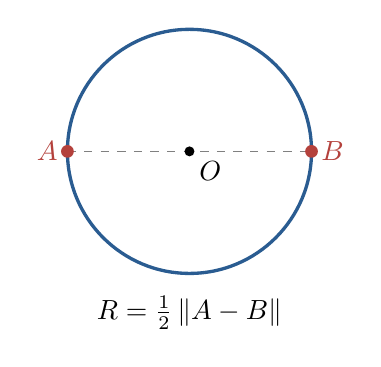
\begin{tikzpicture}[scale=1.0]
  \draw[very thick,mainblue] (0,0) circle (1.55);
  \draw[dashed,gray] (-1.55,0)--(1.55,0);
  \fill[mainred] (-1.55,0) circle (2.3pt) node[left] {$A$};
  \fill[mainred] (1.55,0) circle (2.3pt) node[right] {$B$};
  \fill (0,0) circle (1.8pt) node[below right] {$O$};
  \node at (0,-2.05) {$R=\frac12\norm{A-B}$};
\end{tikzpicture}
\caption{两个支撑点决定直径圆。}
\end{subfigure}
\hfill
\begin{subfigure}[b]{0.44\textwidth}
\centering
\begin{tikzpicture}[scale=1.0]
  \draw[very thick,maingreen] (0,0) circle (1.55);
  \foreach \ang/\lab in {90/A,210/B,330/C}{
    \coordinate (p\lab) at (\ang:1.55);
    \fill[mainred] (p\lab) circle (2.3pt) node[shift={(\ang:0.35)}] {$\lab$};
  }
  \draw[dashed,gray] (pA)--(pB)--(pC)--cycle;
  \fill (0,0) circle (1.8pt) node[below right] {$O$};
  \node at (0,-2.05) {$O$ 为三角形外心};
\end{tikzpicture}
\caption{三个支撑点决定外接圆。}
\end{subfigure}
\caption{二维最小包围圆的两种决定结构。}
\label{fig:mec-support}
\end{figure}

\subsection{圆外新点为何必须成为新的支撑点}

\begin{lemma}[圆外点支撑性]
设 $C$ 为点集 $S$ 的最小包围圆，加入新点 $P\notin C$ 后，新点集 $S\cup\{P\}$ 的最小包围圆必满足 $P$ 位于圆周上。
\label{lem:outside-support}
\end{lemma}
\begin{proof}
反设 $P$ 严格位于新最小圆 $C'$ 内部，则 $P$ 不是 $C'$ 的支撑点。由\cref{thm:mec-support}，$C'$ 可完全由原集合 $S$ 中至多三个圆周点决定。因此仅对 $S$ 而言也需要半径至少为 $R(C')$ 的圆，即 $R(C)\ge R(C')$。另一方面增加点不会使最小包围半径减小，故 $R(C')\ge R(C)$，于是二者半径相等。欧氏平面有限点集的最小包围圆唯一，从而 $C'=C$，但 $P\notin C$，矛盾。故 $P$ 必在 $C'$ 圆周上。
\end{proof}

\subsection{Welzl 递归算法}

\begin{algorithm}[htbp]
\caption{Welzl 随机增量最小包围圆}
\label{alg:welzl}
\begin{algorithmic}[1]
\Require 点集 $P$；已知必须位于圆周上的支撑点集 $R$，且 $|R|\le3$
\Ensure 覆盖 $P\cup R$ 且使 $R$ 位于圆周上的最小圆
\Function{Welzl}{$P,R$}
    \If{$P=\varnothing$ \textbf{or} $|R|=3$}
        \State \Return 由 $R$ 确定的最小圆
    \EndIf
    \State 从 $P$ 中随机选取一点 $p$
    \State $C\gets\Call{Welzl}{P\setminus\{p\},R}$
    \If{$p\in C$}
        \State \Return $C$
    \Else
        \State \Return $\Call{Welzl}{P\setminus\{p\},R\cup\{p\}}$
    \EndIf
\EndFunction
\end{algorithmic}
\end{algorithm}

\subsection{Welzl 正确性证明}

\begin{theorem}[Welzl 正确性]
\cref{alg:welzl} 返回输入点集的全局最小包围圆。
\end{theorem}
\begin{proof}
对 $|P|$ 归纳。基础情形 $P=\varnothing$ 或 $|R|=3$ 时圆由边界约束直接确定。归纳步骤中随机取 $p\in P$，先求
\[
C=\MEC(P\setminus\{p\},R).
\]
若 $p\in C$，则 $C$ 已覆盖全部点；若存在更小圆覆盖 $P\cup R$，它也会覆盖 $(P\setminus\{p\})\cup R$，与 $C$ 的最小性矛盾。若 $p\notin C$，由\cref{lem:outside-support}，$p$ 必成为新最小圆的支撑点，因此原问题等价于
\[
\MEC(P\setminus\{p\},R\cup\{p\}).
\]
根据归纳假设第二次递归返回正确答案，故算法正确。
\end{proof}

\subsection{Welzl 期望时间复杂度}

定义 $T_r(n)$ 为已经固定 $r$ 个支撑点时，对另外 $n$ 个随机排列点运行 Welzl 所需的期望时间，其中 $r=0,1,2,3$。当 $r=3$ 时立即结束，故
\begin{equation}
T_3(n)=O(1).
\end{equation}
一般地，最终圆最多还需要 $3-r$ 个新的支撑点。因此在随机顺序下，当前最后一个点恰好属于这些决定性支撑点的概率不超过
\begin{equation}
\frac{3-r}{n}.
\end{equation}
于是有递推上界
\begin{equation}
T_r(n)
\le
T_r(n-1)+O(1)+\frac{3-r}{n}T_{r+1}(n-1).
\label{eq:welzl-rec-complexity}
\end{equation}
从 $r=2$ 开始向上代入：
\begin{align}
T_2(n)&\le T_2(n-1)+O(1)+\frac1nO(1)=O(n),\\
T_1(n)&\le T_1(n-1)+O(1)+\frac2nO(n)=O(n),\\
T_0(n)&\le T_0(n-1)+O(1)+\frac3nO(n)=O(n).
\end{align}
故
\begin{equation}
\boxed{\mathbb E[T_{\rm MEC}(m)]=O(m)}.
\end{equation}
随机化三层迭代实现的最坏情况仍可达到 $O(m^3)$，但随机打乱后具有上述期望线性复杂度。若采用迭代形式，除输入点外额外空间为 $O(1)$；递归实现需要 $O(m)$ 的调用栈。

% ============================================================
\section{直径圆覆盖判据}
% ============================================================

旋转卡壳得到区域直径 $D$，Welzl 得到最小覆盖半径 $R^*$。下面建立二者之间的严格判定关系。

\begin{theorem}[直径圆覆盖判据]
存在一个直径恰为 $D$ 的圆覆盖定位区域 $\Omega$，当且仅当
\begin{equation}
\boxed{R^*=\frac{D}{2}}.
\label{eq:cover-iff}
\end{equation}
等价地，定义
\begin{equation}
\rho=\frac{2R^*}{D},
\label{eq:rho}
\end{equation}
则覆盖成立当且仅当 $\rho=1$。
\end{theorem}
\begin{proof}
设 $P,Q\in\Omega$ 为直径点，$\norm{P-Q}=D$。任意能够覆盖 $\Omega$ 的圆若圆心为 $O$、半径为 $R$，则
\begin{align}
D=\norm{P-Q}
&\le\norm{P-O}+\norm{O-Q}\\
&\le2R.
\end{align}
故所有覆盖圆均满足
\begin{equation}
R\ge\frac D2,
\end{equation}
特别地 $R^*\ge D/2$。

若存在直径为 $D$ 的覆盖圆，其半径正好为 $D/2$，故 $R^*\le D/2$；结合前式得 $R^*=D/2$。反之，若 $R^*=D/2$，则最小包围圆自身直径即为 $D$，它显然覆盖 $\Omega$。因此\cref{eq:cover-iff} 成立。
\end{proof}

\begin{figure}[htbp]
\centering
\begin{tikzpicture}[scale=1.1]
  \coordinate (B) at (-1.8,0);
  \coordinate (C) at (1.8,0);
  \coordinate (A) at (0,2.2);
  \fill[mainblue!8] (A)--(B)--(C)--cycle;
  \draw[thick] (A)--(B)--(C)--cycle;
  \draw[dashed,very thick,mainorange] (0,0) circle (1.8);
  \draw[very thick,maingreen] (0,0.364) circle (1.836);
  \fill[mainred] (A) circle (2.4pt) node[above] {$A$};
  \fill[mainred] (B) circle (2.4pt) node[below left] {$B$};
  \fill[mainred] (C) circle (2.4pt) node[below right] {$C$};
  \draw[mainblue,very thick] (B)--(C) node[midway,below] {最长边 $D$};
  \node[mainorange!80!black,align=left] at (4.0,0.65) {橙色虚线：\\以 $BC$ 为直径的圆\\半径 $D/2$，未覆盖 $A$};
  \node[maingreen!70!black,align=left] at (4.0,-0.65) {绿色实线：\\最小包围圆\\半径 $R^*>D/2$};
\end{tikzpicture}
\caption{为什么“最远点对的直径圆”不一定覆盖整个区域。对于锐角三角形，最小包围圆由三个顶点共同决定，因此 $2R^*/D>1$。}
\label{fig:diameter-circle-fail}
\end{figure}

\subsection{Jung 定理给出的数值校验区间}

平面 Jung 定理给出任意直径为 $D$ 的平面点集均可被半径 $D/\sqrt3$ 的圆覆盖，因此
\begin{equation}
\frac D2\le R^*\le\frac D{\sqrt3}.
\end{equation}
故
\begin{equation}
\boxed{1\le\rho\le\frac2{\sqrt3}\approx1.1547.}
\label{eq:rho-range}
\end{equation}
该区间可作为程序结果的强一致性检查：若计算得到明显的 $\rho<1$ 或 $\rho>2/\sqrt3$，通常意味着 HPI、直径、MEC 或浮点误差处理存在问题。

% ============================================================
\section{完整求解算法与复杂度}
% ============================================================

\begin{algorithm}[htbp]
\caption{定位区域直径与覆盖性判定的完整算法}
\label{alg:full}
\begin{algorithmic}[1]
\Require 检测点 $S_i$、示向角 $\theta_i$、误差上限 $\eps$
\Ensure 定位区域顶点、区域直径 $D$、最小覆盖圆 $(O^*,R^*)$、覆盖判据 $\rho$
\State \textbf{角域建模：} 对每个检测点构造 $\theta_i\pm\eps$ 两条边界并转化为左半平面
\State \textbf{区域恢复：} 调用\cref{alg:hpi} 得到凸多边形顶点 $V_1,\ldots,V_m$
\State \textbf{直径计算：} 调用\cref{alg:calipers} 得到 $D$
\State \textbf{最小覆盖圆：} 随机打乱 $V_1,\ldots,V_m$，调用\cref{alg:welzl} 得到 $(O^*,R^*)$
\State $\rho\gets 2R^*/D$
\If{$\abs{\rho-1}\le\eps_{\rm num}$}
    \State 判定：存在直径为 $D$ 的圆覆盖定位区域
\Else
    \State 判定：不存在直径为 $D$ 的圆覆盖定位区域
\EndIf
\State \Return $(V_1,\ldots,V_m),D,O^*,R^*,\rho$
\end{algorithmic}
\end{algorithm}

设输入半平面数为 $n$，最终凸多边形顶点数为 $m$，显然 $m\le n$。各阶段复杂度见\cref{tab:complexity}。

\begin{table}[htbp]
\centering
\caption{各算法阶段复杂度}
\label{tab:complexity}
\begin{tabular}{lll}
\toprule
阶段 & 时间复杂度 & 主要原因 \\
\midrule
半平面方向角排序 & $O(n\log n)$ & 比较排序 \\
HPI 双端队列维护 & $O(n)$ & 每条边最多入队、出队各一次 \\
旋转卡壳 & $O(m)$ & 两个循环指针均只前进一圈 \\
Welzl 最小包围圆 & $\mathbb E[O(m)]$ & 随机增量倒推分析 \\
\midrule
总体 & $\boxed{\mathbb E[O(n\log n)]}$ & $m\le n$，排序占主导 \\
\bottomrule
\end{tabular}
\end{table}

因此总时间复杂度为
\begin{equation}
\boxed{
\mathbb E[T(n,m)]
=O(n\log n)+O(m)+\mathbb E[O(m)]
=O(n\log n).
}
\end{equation}

% ============================================================
\section{数值实现细节与边界情形}
% ============================================================

\subsection{浮点容差}

计算几何中不建议直接使用严格的 $=0$ 比较。设置
\[
\eps_{\rm num}=10^{-9}
\]
（或根据坐标量级进行缩放），并使用：
\begin{itemize}
  \item 半平面判断：$\bm d\cross(P-S)\ge-\eps_{\rm num}$；
  \item 平行判断：$\abs{\bm d_1\cross\bm d_2}<\eps_{\rm num}$；
  \item 圆内判断：$\norm{P-O}^2\le R^2+\eps_{\rm num}$；
  \item 覆盖判定：$\abs{2R^*/D-1}\le\eps_{\rm num}$。
\end{itemize}

\subsection{角度制转换}

若题面以“正北为 $0^\circ$、顺时针为正”给出示向度，而程序采用“$x$ 轴正方向为 $0$、逆时针为正”的数学角，则需要预先转换，例如
\begin{equation}
\alpha=\frac{\pi}{2}-\beta,
\end{equation}
并将结果归一化到 $[0,2\pi)$。

\subsection{目标区域圆先验的处理}

若题目还给出干扰源必须位于圆形目标区域
\begin{equation}
B(O_0,R_0)=\{P:\norm{P-O_0}\le R_0\},
\end{equation}
则严格可行域应为
\begin{equation}
\Omega^*=\left(\bigcap_jH_j\right)\cap B(O_0,R_0).
\label{eq:target-disk}
\end{equation}
先执行 HPI 得到多边形 $\Omega$。若所有顶点均满足 $\norm{V_i-O_0}\le R_0$，则由圆盘的凸性有 $\Omega\subseteq B(O_0,R_0)$，圆先验不活跃，本文全部算法可直接使用。

若存在顶点落在目标圆外，则 $\Omega^*$ 的边界可能包含圆弧，此时不能简单用目标圆的外接正方形替代圆盘，也不能只对原多边形顶点运行旋转卡壳与 Welzl。此类情形应单独加入线圆交点与圆弧极值分析，或采用能够显式处理圆弧边界的凸优化/计算几何方法。

% ============================================================
\section{结论}
% ============================================================

本问可被统一表述为“\textbf{凸可行域恢复 + 凸集极值计算}”。首先将每个带误差的示向角严格转化为两个线性半平面，并利用方向角排序与双端队列求取其交，从而以 $O(n\log n)$ 时间恢复定位凸多边形。HPI 的正确性来自凸集被新半平面切割时只会连续删除一段边界，而方向角排序保证该失效链在线性 deque 中只能出现在两端。

在此基础上，利用旋转卡壳遍历所有对踵关系，以 $O(m)$ 时间得到区域直径 $D$；再由凸多边形最小覆盖圆等价于顶点集合最小包围圆，并利用二维 MEC 至多由三个支撑点决定的性质，采用 Welzl 随机增量算法在期望 $O(m)$ 时间内得到最小覆盖半径 $R^*$。最终通过
\[
\boxed{\rho=\frac{2R^*}{D}}
\]
进行覆盖判定：$\rho=1$ 当且仅当存在直径为 $D$ 的圆完整覆盖定位区域。故完整方法在保持严格几何正确性的同时，总体期望时间复杂度仍为
\[
\boxed{O(n\log n)}.
\]

\end{document}
